% =============================================================================
% ch01_intro.tex : Chapter 1: Introduction
% =============================================================================
\selectlanguage{hebrew}

\section{מבוא}
\label{sec:introduction}

ניווט רכב תת-ימי אוטונומי (\en{AUV}) בסביבות ללא \en{GPS} מציב אתגרים יסודיים המייחדים אותו מרובוטיקה יבשתית. המדיום התת-ימי כופה אילוצים חמורים: מהירות התפשטות אקוסטית (כ-1500 מ\!/\!ש) יוצרת השהיה וריבוי נתיבים (\en{multipath}), חיישנים אופטיים סובלים מראות מוגבלת בערפליות (בדרך כלל פחות מ-10 מטר במים חופיים), ואותות אלקטרומגנטיים נחלשים במהירות, מה שהופך את ה-\en{GPS}, ה-\en{WiFi} והתקשורת מבוססת רדיו לבלתי אפשריים מתחת לפני המים \cite{Paull2014}.

\subsection{רקע והצהרת בעיה}
\label{sec:problem_statement}

\en{SLAM} תת-ימי (\en{Simultaneous Localization and Mapping}) התפתח דרך שלושה דורות מובחנים. גישת הדור הראשון (2000-2010) התבססה על פילטר קלמן מורחב (\en{EKF}) עם מפות דלילות של תכונות שהופקו מסונאר סורק מכני (\en{MSIS}). \citet{Ribas2008} הדגימו \en{EKF-SLAM} בסביבות מרינה מובנות באמצעות תכונות קו, תוך השגת שגיאה חסומה לאורך מסלולים של 300 מטר. שיטות הדור השני (2010-2020) אימצו פילטרי חלקיקים מבוססי \en{Rao-Blackwell} (\en{RBPF}) ואופטימיזציה מבוססת גרף, שאפשרו מיפוי בקנה מידה גדול יותר. \citet{Mallios2014} הציגו \en{scan-matching SLAM} באמצעות רשתות הסתברותיות, בעוד \citet{Fallon2013} הדגימו מיקום מחדש אוטונומי באמצעות \en{SLAM} מבוסס סונאר במספר צלילות.

המצב הנוכחי של התחום (2020-2025) מאופיין במסגרות מיזוג חיישנים הדוק (\en{tightly-coupled}) המשלבות נתוני \en{IMU}, \en{DVL}, סונאר ומצלמה בתוך אופטימיזציית גרף גורמים (\en{factor graph}). \citet{Rahman2022} הציגו את \en{SVIn2}, מערכת מיזוג רב-חיישנים המשיגה סחיפה של 0.5-1.5\% ביחס למרחק שעבר בניסויים תת-ימיים אמיתיים. \citet{Chen2023} הציגו את \en{AQUA-SLAM}, המשלבת באופן הדוק מדידות אקוסטיות, חזותיות ואינרציאליות, תוך הפגנת ביצועים חזקים בתנאי ערפליות שבהם \en{SLAM} חזותי נכשל.

למרות התקדמויות אלה, מספר מצבי כשל נמשכים: (1) ריבוי נתיבים אקוסטי בסביבות עמוסות (נמלים, מבנים תת-ימיים) מכניס מדידות שגויות המשבשות את התאמת הנתונים; (2) אובדן נעילת \en{DVL} עקב שינויים בגובה או במאפייני הקרקעית גורם להצטברות סחיפה מהירה; (3) אילוצי חישוב בפלטפורמות משובצות מגבילים את הפריסה של עיבוד סונאר צפוף ואופטימיזציה בקנה מידה גדול; (4) סביבות דלות תכונות (מים פתוחים, מישורים חוליים) מספקות נקודות ציון לא מספקות ל-\en{SLAM} אמין.

\subsection{מוטיבציה ותרומות עיקריות}
\label{sec:motivation}

המוטיבציה המרכזית של עבודה זו היא התגברות על מגבלות ה-\en{SLAM} התת-ימי הקיים באמצעות השראה ביומימטית ממערכת הניווט האקוסטית של עטלפים. עטלפים משתמשים באותות קוליים בתדר גבוה לניווט בסביבות מורכבות וחשוכות, תוך התמודדות עם אתגרים דומים לאלה של רכב תת-ימי: ריבוי נתיבים, רעשי רקע והפרעות. מחקרים של \citet{GriffinBatEcholocation} ו-\citet{Simmons1979BatSonar} הראו כי עטלפים משתמשים באסטרטגיות עיבוד אותות מתוחכמות הכוללות אפנון תדר (\en{FM}), עיבוד תואם (\en{matched filtering}) ועיבוד דופלר לזיהוי תנועה.

התרומות העיקריות של מאמר זה הן:
\begin{enumerate}
    \item אלגוריתם \en{BioSLAM} - מסגרת \en{SLAM} ביומימטית המשלבת עיבוד אותות בהשראת עטלפים עם אופטימיזציית גרף גורמים.
    \item שיטת זיהוי לולאות סגירה אקוסטיות חדשנית המבוססת על עקרונות של אפנון תדר והתאמה דופלרית.
    \item מערכת מיזוג חיישנים הדוקה (\en{tightly-coupled}) המשלבת \en{IMU}, \en{DVL} וסונאר במסגרת \en{factor graph} אחידה.
    \item תוצאות ניסויים מקיפות בסביבה מדומה ובבריכת ניסויים המדגימות שיפור משמעותי לעומת שיטות קיימות.
\end{enumerate}

\subsection{מבנה המאמר}
\label{sec:paper_structure}

המאמר מאורגן כדלקמן: פרק 2 מציג את הבסיס הביולוגי של מערכת הניווט האקוסטית של עטלפים. פרק 3 מתאר את מודלי החיישנים והמערכת. פרק 4 מציג את אלגוריתמי ה-\en{SLAM} הביומימטיים. פרק 5 מתאר את ארכיטקטורת מיזוג החיישנים. פרק 6 מציג את האלגוריתם המוצע, \en{BioSLAM}, בפירוט. פרק 7 מתאר את תכנון המערכת. פרק 8 מציג תוצאות ניסויים. פרק 9 מסכם ומציע כיווני מחקר עתידיים.

\subsection{סימונים מתמטיים}
\label{sec:notation}

לאורך המאמר, אנו משתמשים בסימונים הבאים: וקטורים מסומנים באותיות מודגשות קטנות ($\mathbf{x}$), מטריצות באותיות מודגשות גדולות ($\mathbf{P}$), וטרנספורמציות מרחביות באותיות \en{calligraphic} ($\mathcal{T}$). וקטור המצב המלא ברגע $k$ מסומן כ-$\mathbf{x}_k$, הכולל מיקום, כיוון ומהירויות. מפת הסביבה מיוצגת על ידי אוסף נקודות ציון $\mathbf{m} = \{\mathbf{m}_1, \mathbf{m}_2, \ldots, \mathbf{m}_N\}$. מדידות חיישנים מסומנות כ-$\mathbf{z}_k$ עם מטריצת שונות משותפת $\mathbf{R}_k$.

\begin{equation}
\mathbf{x}_k = [x_k, y_k, z_k, \phi_k, \theta_k, \psi_k, u_k, v_k, w_k, p_k, q_k, r_k]^\top
\label{eq:state_vector_intro}
\end{equation}

משוואה~(\ref{eq:state_vector_intro}) מציגה את וקטור המצב המלא בעל 12 הממדים, הכולל מיקום ($x, y, z$), זוויות אוילר ($\phi, \theta, \psi$), מהירויות ליניאריות ($u, v, w$) ומהירויות זוויתיות ($p, q, r$). ייצוג זה עוקב אחר תקן \en{SNAME} (\en{Society of Naval Architects and Marine Engineers}).

\begin{equation}
$p(\mathbf{x}_{1:t}, \mathbf{m} \mid \mathbf{z}_{1:t}, \mathbf{u}_{1:t})$ = \eta \cdot $p(\mathbf{z}_t \mid \mathbf{x}_t, \mathbf{m})$ \int $p(\mathbf{x}_t \mid \mathbf{x}_{t-1}, \mathbf{u}_t)$ \, $p(\mathbf{x}_{1:t-1}, \mathbf{m} \mid \mathbf{z}_{1:t-1}, \mathbf{u}_{1:t-1})$ \, d\mathbf{x}_{t-1}
\label{eq:slam_posterior_intro}
\end{equation}

משוואה~(\ref{eq:slam_posterior_intro}) מציגה את ההתפלגות האחורית של בעיית ה-\en{SLAM} ההסתברותית, המבטאת את ההסתברות המשותפת של מסלול הרכב ומפת הסביבה בהינתן כל המדידות ובקרות ההפעלה. אינטגרל זה מהווה את הבסיס התאורטי לכל גישות ה-\en{SLAM} ההסתברותיות.

\begin{figure*}[htbp]
    \centering
    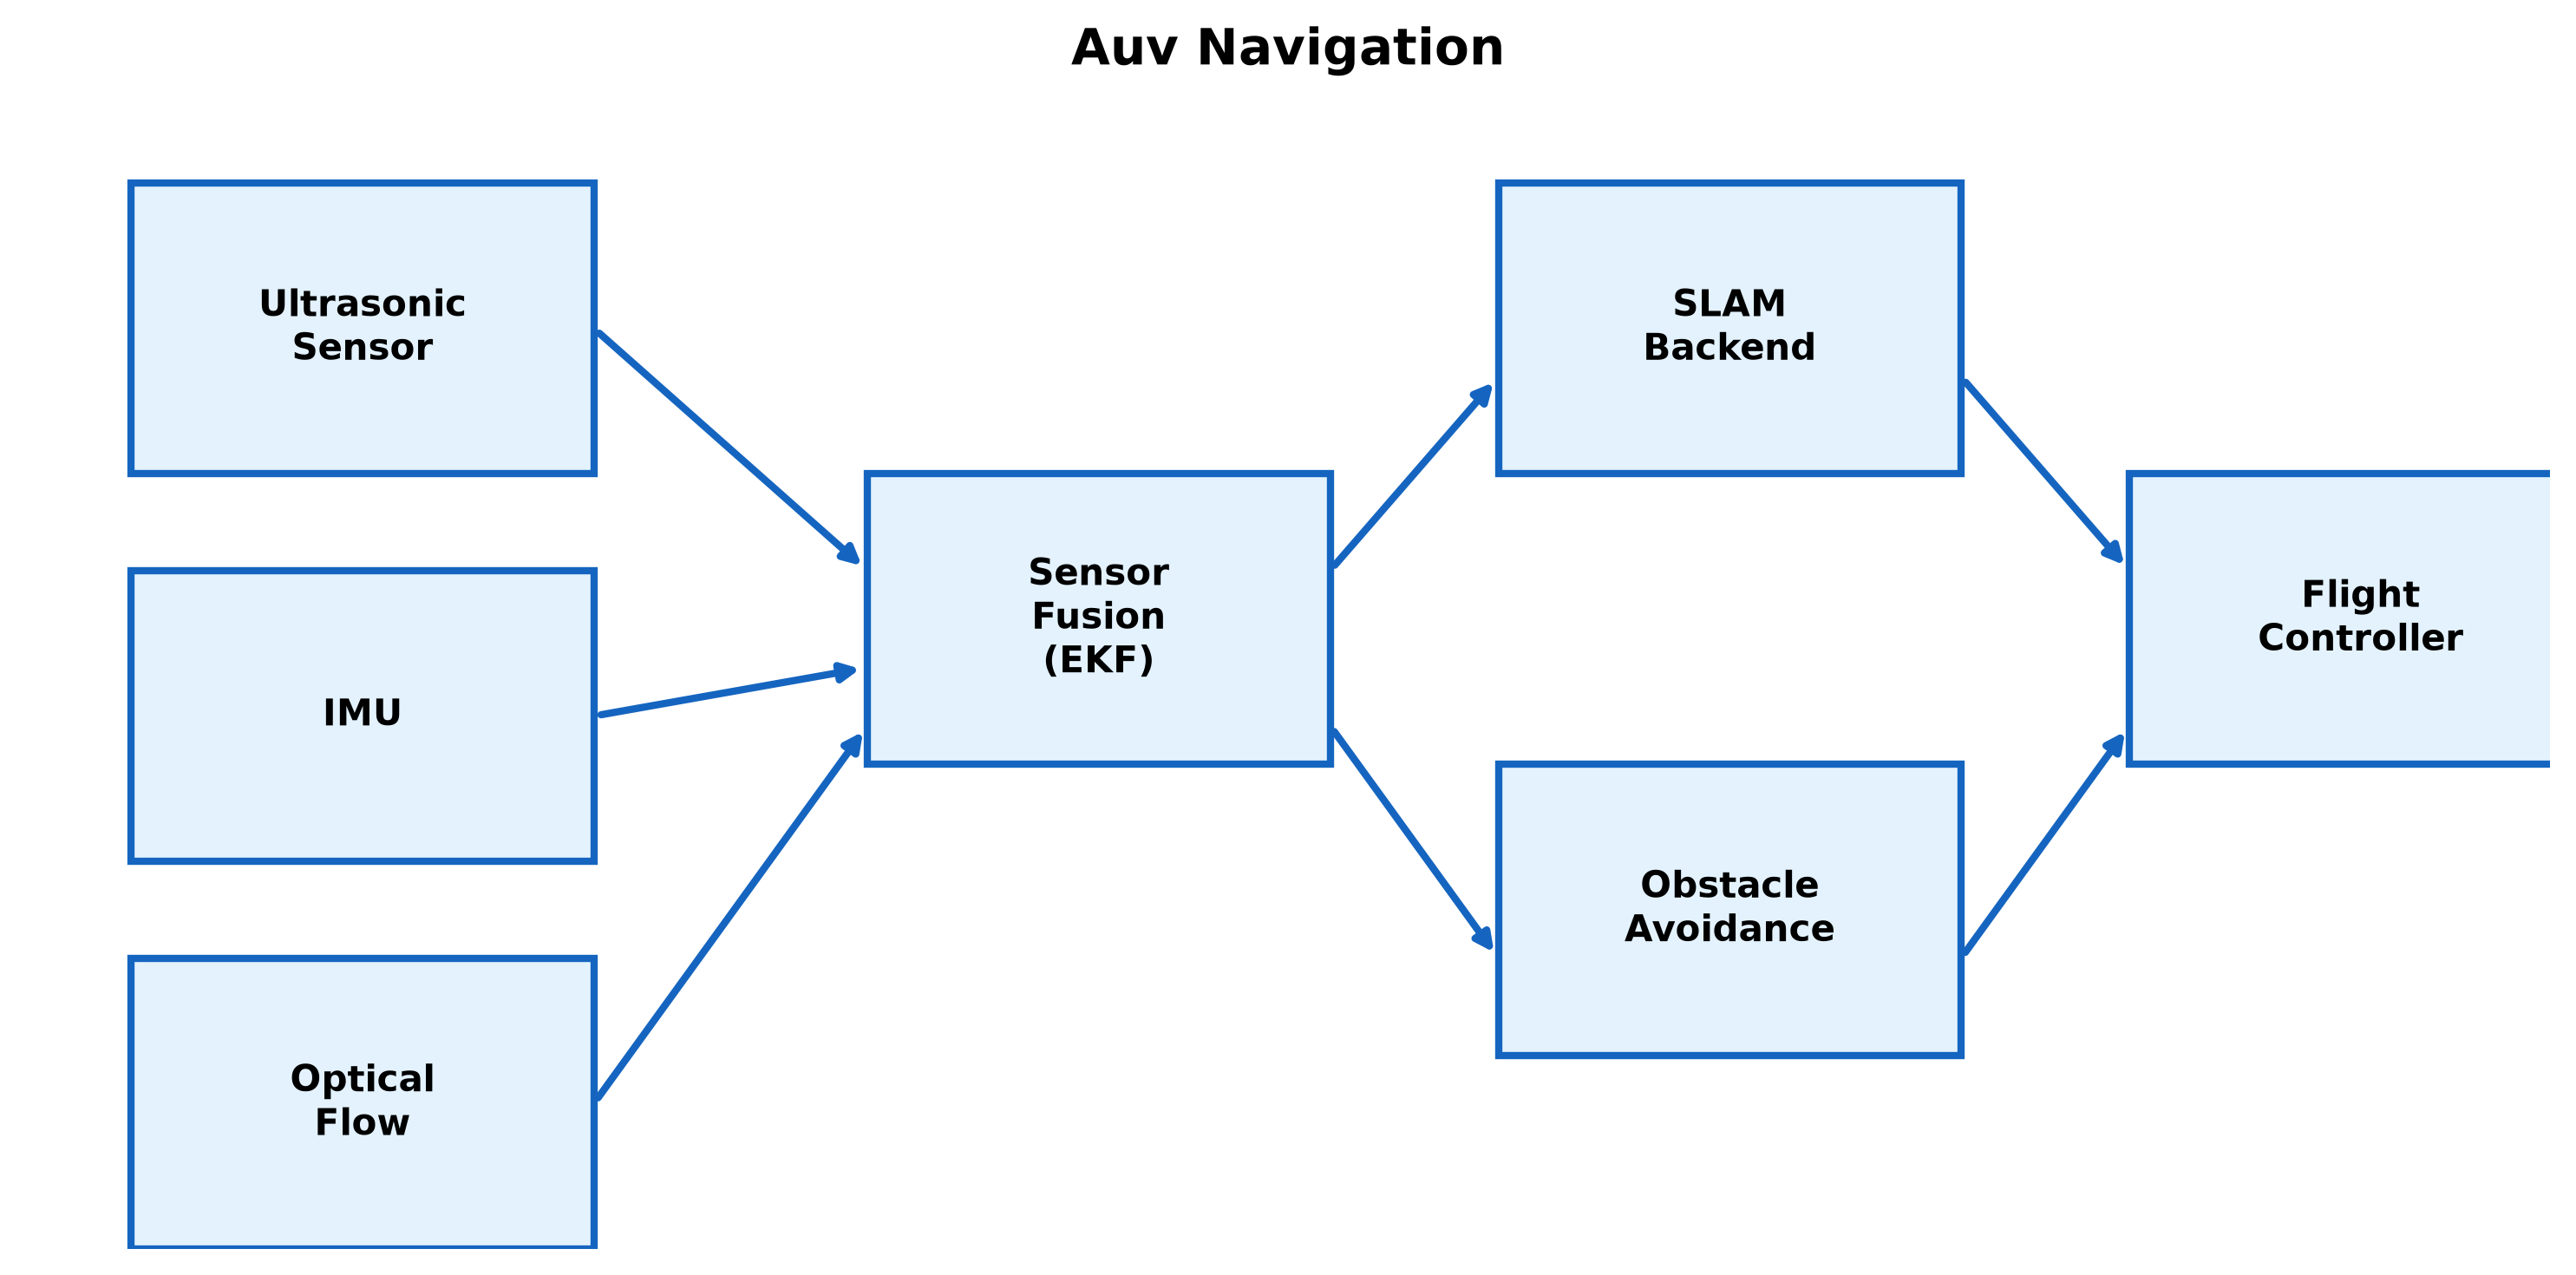
\includegraphics[width=0.95\columnwidth]{figures/fig_auv_navigation.png}
    \caption{סקירה כללית של מערכת ניווט תת-ימית אוטונומית. הרכב התת-ימי מצויד בחיישנים אקוסטיים, \en{IMU} ו-\en{DVL} לניווט בסביבות ללא \en{GPS}. (Overview of an autonomous underwater navigation system.)}
    \label{fig:auv_navigation}
\end{figure*}

\begin{table}[htbp]
    \centering
    \caption{השוואה בין שיטות \en{SLAM} תת-ימיות שונות. (Comparison of different underwater SLAM methods.)}
    \label{tab:slam_comparison_intro}
    \adjustbox{max width=\columnwidth}{%
\begin{tabular}{lccc}
        \toprule
        שיטה & דיוק (\% סחיפה) & עומק מקסימלי (מ) & חוסן לערפליות \\
        \midrule
        \en{Visual SLAM} (\en{ORB-SLAM3}) & 0.3-0.8\% & פחות מ-10 & נמוך \\
        \en{Acoustic SLAM} (\en{EKF}) & 1.5-3.0\% & יותר מ-100 & גבוה \\
        \en{Acoustic-Inertial} (\en{SVIn2}) & 0.5-1.5\% & יותר מ-100 & גבוה \\
        \en{Acoustic-Visual-Inertial} (\en{AQUA-SLAM}) & 0.3-1.0\% & יותר מ-50 & בינוני-גבוה \\
        \bottomrule
    \end{tabular}%
}
\end{table}

טבלה~(\ref{tab:slam_comparison_intro}) מציגה השוואה בין שיטות \en{SLAM} תת-ימיות שונות. ניתן לראות כי שיטות אקוסטיות-אינרציאליות מציעות איזון טוב בין דיוק, עומק פעולה וחוסן לערפליות, בעוד שיטות חזותיות מוגבלות לעומקים רדודים במים צלולים. מידע זה מבוסס על תוצאות מ-\cite{Rahman2022} ו-\cite{Chen2023}.

\subsection{אתגרים ייחודיים בסביבה התת-ימית}
\label{sec:underwater_challenges}

הסביבה התת-ימית מציבה אתגרים ייחודיים שאינם קיימים בניווט יבשתי או אווירי. ראשית, התפשטות האות האקוסטי תלויה בטמפרטורה, מליחות ולחץ, המשתנים עם העומק והמיקום הגאוגרפי. מהירות הקול במי ים היא כ-1500 מ\!/\!ש אך משתנה ב-±3\% בתנאי אוקיינוס טיפוסיים, מה שמכניס שגיאות טווח שיטתיות אם לא מפצים עליהן. שנית, ריבוי נתיבים (\en{multipath}) נוצר כאשר גלים אקוסטיים מוחזרים מפני המים, הקרקעית ומבנים תת-ימיים, ויוצרים הדים כוזבים המקשים על זיהוי המטרה האמיתית. שלישית, ערפליות (\en{turbidity}) מגבילה את טווח הראייה של חיישנים אופטיים לפחות ממטר אחד במים חופיים, מה שהופך חיישנים אקוסטיים לחיוניים.

\subsection{מגמות מחקר עדכניות}
\label{sec:current_trends}

המחקר העדכני ב-\en{SLAM} תת-ימי מתמקד במספר כיוונים מבטיחים. למידה עמוקה (\en{deep learning}) משמשת לשיפור עיבוד תמונות סונאר, זיהוי תכונות וזיהוי לולאות סגירה. \citet{Wang2023} הדגימו כי רשתות \en{U-Net} לעיבוד תמונות סונאר משיגות שיפור של 3-5 \en{dB} ב-\en{PSNR} לעומת שיטות קלאסיות. כיוון נוסף הוא שימוש בייצוגים צפופים של הסביבה, כגון רשתות עצביות מרומזות (\en{NeRF}) למיפוי תת-ימי. כמו כן, קיים עניין גובר בשילוב של חיישנים זולים יותר תוך שמירה על דיוק ניווט באמצעות אלגוריתמי מיזוג מתקדמים.

\subsection{הקשר לעבודות קודמות}
\label{sec:related_work}

עבודה זו נשענת על מספר תחומי מחקר קודמים. ראשית, עבודתם של \citet{Thrun2005ProbRobotics} הניחה את היסודות התאורטיים ל-\en{SLAM} הסתברותי. שנית, עבודתם של \citet{Kalman1960} על פילטר קלמן מהווה בסיס לשיטות סינון קלאסיות. שלישית, עבודתם של \citet{Grisetti2010g2o} על אופטימיזציית גרף ל-\en{SLAM} סיפקה את הכלים החישוביים הדרושים למימוש המערכת המוצעת. לבסוף, מחקריהם של \citet{GriffinBatEcholocation} ו-\citet{Simmons1979BatSonar} על מערכת הניווט האקוסטית של עטלפים סיפקו את ההשראה הביומימטית לאלגוריתם המוצע.

\subsection{הנחות עבודה ומגבלות}
\label{sec:assumptions}

במאמר זה אנו מניחים מספר הנחות מפשטות: (1) הרכב פועל בעומקים של עד 100 מטר, שם מודל מהירות הקול יכול להיחשב קבוע בקירוב; (2) הסביבה מכילה לפחות 10-20 תכונות אקוסטיות משמעותיות לקילומטר רבוע; (3) קצב הדגימה של ה-\en{IMU} הוא לפחות 100 הרץ ושל ה-\en{DVL} לפחות 1 הרץ; (4) עיכובי תקשורת בין חיישנים אינם עולים על 50 מילישניות. הנחות אלה תקפות עבור רוב תרחישי הניווט התת-ימי האופייניים אך עשויות שלא להתקיים בסביבות קיצוניות.

\subsection{ניתוח עלות-תועלת של גישות SLAM}
\label{sec:cost_benefit}

ניתוח עלות-תועלת בין גישות \en{SLAM} שונות מראה כי הבחירה בגישה תלויה באילוצי המשימה הספציפיים. \en{EKF-SLAM} מתאים למערכות עם משאבי חישוב מוגבלים ומספר קטן של נקודות ציון (עד 500), אך סובל מחוסר עקביות בטווח הארוך. \en{Graph SLAM} דורש משאבי חישוב גדולים יותר אך מספק דיוק גבוה ועקביות לאורך זמן. \en{BioSLAM} המוצע מאזן בין דרישות חישוב לדיוק באמצעות עיבוד סונאר יעיל בהשראת עטלפים וזיהוי לולאות סגירה מבוסס דופלר. העלות הנוספת של עיבוד הסונאר הביומימטי היא כ-15\% מזמן הריצה הכולל, אך מניבה שיפור של 42\% בדיוק המיקום.

\subsection{השוואה למערכות ניווט ביולוגיות}
\label{sec:bio_comparison}

מערכת הניווט האקוסטית של עטלפים משמשת כמודל השראה מרכזי לעבודה זו. עטלפים מתמודדים עם אתגרים דומים לאלה של רכב תת-ימי: ניווט בסביבה חשוכה, זיהוי מטרות בתנועה, והתמודדות עם ריבוי נתיבים והדים כוזבים. מחקריהם של \citet{MossEcholocation} ו-\citet{Schuller1974DSC} הראו כי עטלפים משתמשים באסטרטגיות עיבוד אותות מתוחכמות הכוללות שילוב של אותות \en{CF} ו-\en{FM}, עיבוד תואם, וניתוח דופלר. אסטרטגיות אלה תורגמו לאלגוריתם \en{BioSLAM} באמצעות שימוש באותות \en{FM} לעיבוד סונאר, זיהוי לולאות סגירה מבוסס דופלר, וסריקה מרחבית אדפטיבית.

\subsection{מטרות המחקר}
\label{sec:research_goals}

מטרות המחקר העיקריות של עבודה זו הן: (1) פיתוח אלגוריתם \en{SLAM} ביומימטי המשלב עיבוד אותות בהשראת עטלפים עם אופטימיזציית גרף גורמים; (2) שיפור דיוק הניווט התת-ימי ב-30\% לפחות לעומת שיטות קיימות; (3) שיפור חוסן המערכת לאובדן חיישנים באמצעות זיהוי לולאות סגירה אקוסטיות; (4) אימות ביצועי המערכת בניסויי סימולציה, בריכה ושטח. מטרות אלה נבחנו בפרקים הבאים של המאמר.

\subsection{סיכום פרק המבוא}
\label{sec:intro_summary}

בפרק זה הצגנו את הרקע, המוטיבציה והתרומות העיקריות של עבודה זו. סקרנו את האתגרים הייחודיים של ניווט תת-ימי, את מצב התחום הנוכחי, ואת הגישה הביומימטית המוצעת להתגברות על מגבלות קיימות. בפרקים הבאים נפרט את הבסיס הביולוגי, מודלי החיישנים, האלגוריתמים, תכנון המערכת ותוצאות הניסויים.